\chapter{Security Analysis}\label{chap:security_analysis}

\section{Attack landscape}

In this section, we give an overview of the various attacks that we consider for our model.

\subsection{Enclave attacks}

Most SGX attacks are side-channel \cite{sgx_survey} attacks, i.e. attacks that are based on information gained from the implementation of the system under attack, rather than weaknesses in the implementation itself. Popular side-channel attacks against SGX are cache-based timing attacks, such as \textit{Flush+Reload} \cite{flush_reload} or \textit{Prime+Probe} \cite{prime_probe}. Both attacks exploit cache behaviour to leak information on victim access to shared memory. In \textit{Flush+Reload}, the attacker flushes a memory line and then measures the time that it takes for the line to be reloaded. If the line was reloaded fast, then the attacker infers that the victim accessed the data located at that line. In \textit{Prime+Probe}, the attacker first primes the cache (i.e. loads it with dummy data) and waits for the victim to access one of the cache lines. Afterwards, the attacker probes the cache and measures its response time. If the access is fast, then the victim did not access this cache line. If it is slow, it did access it. Figure ~\ref{fig:cache} shows how processors fetch data from the cache / memory, and how it relates to access time.

To defend against such attacks, the enclave's authors must make sure that their design is side-channel resilient. This can be achieved by making sure that the code is designed in a cache leakage-free manner, making the execution flow and memory access patterns independent of the data accessed. For other kinds of attacks, \cite{sgx_survey} suggests that authors can act on multiple fronts: microcode patches, system/application design and compiler/SDK. While this is an active and interesting research area, it is mostly independent of the focus of this thesis, and thus we will not explore these attacks further.

\begin{figure}[h!]
	\center
	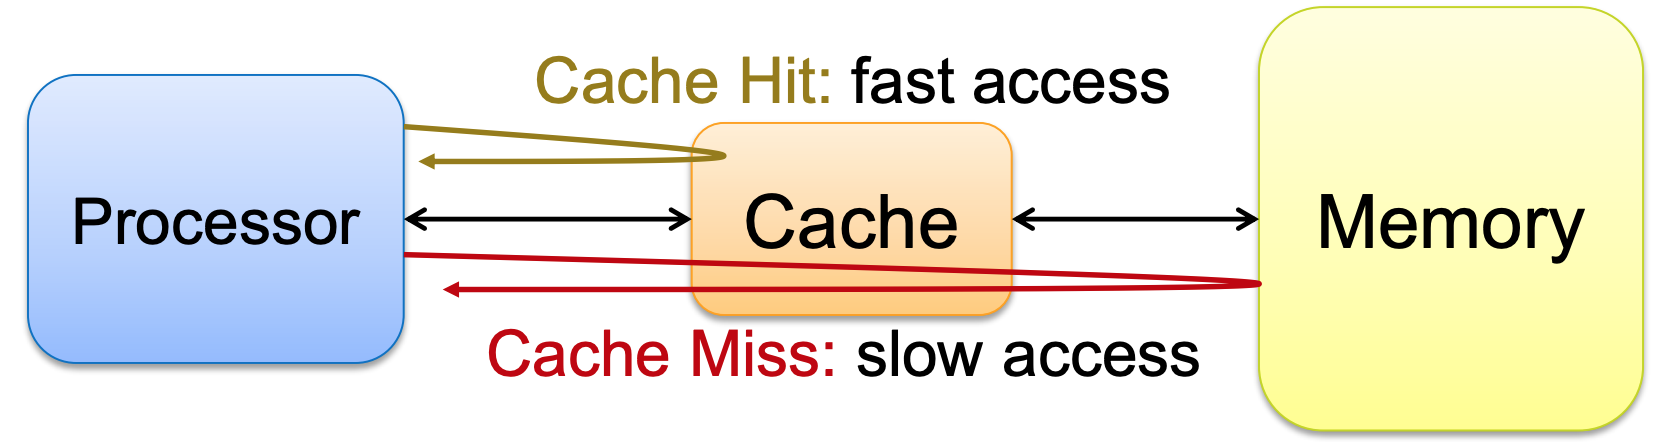
\includegraphics[scale=0.35]{images/introduction/cache}
	\caption{\label{fig:cache} Illustration of a processor fetching data from cache or memory \cite{intel_slides}.}
\end{figure}

\subsection{Security \& privacy attacks}

Since the questionnaires are served to the customers through e.g. a web application, we must consider security attacks targeted at such applications. A malicious customer could try to influence the model accuracy by tempering with the learning set. This could be done by e.g. flooding the web application with bogus questionnaire's answers. In this thesis we will assume that customers are trustworthy, and we will instead focus on privacy attacks, in particular those that target machine learning models.

If a machine learning model was trained using personal data, such as people's health records or identity information, then a privacy attack would aim at extracting these information to benefit the attacking party. For the scope of this thesis, we consider the insurance company to be the adversary, since they own the machine learning model. While they cannot access its content (as it is enclave-protected), it can design privacy attacks in order to gain information about the training set used by the model (i.e. the questionnaires submitted by the customers). Since it is assumed that the model is trained and run within a trusted environment, we will focus our threat model on black-box attacks (i.e. the attacker only has access to the model's API, can submit input vectors and retrieve their corresponding predictions), as shown in Figure ~\ref{fig:threat_model} (adapted from \cite{ml_survey}).

\begin{figure}[h!]
	\center
	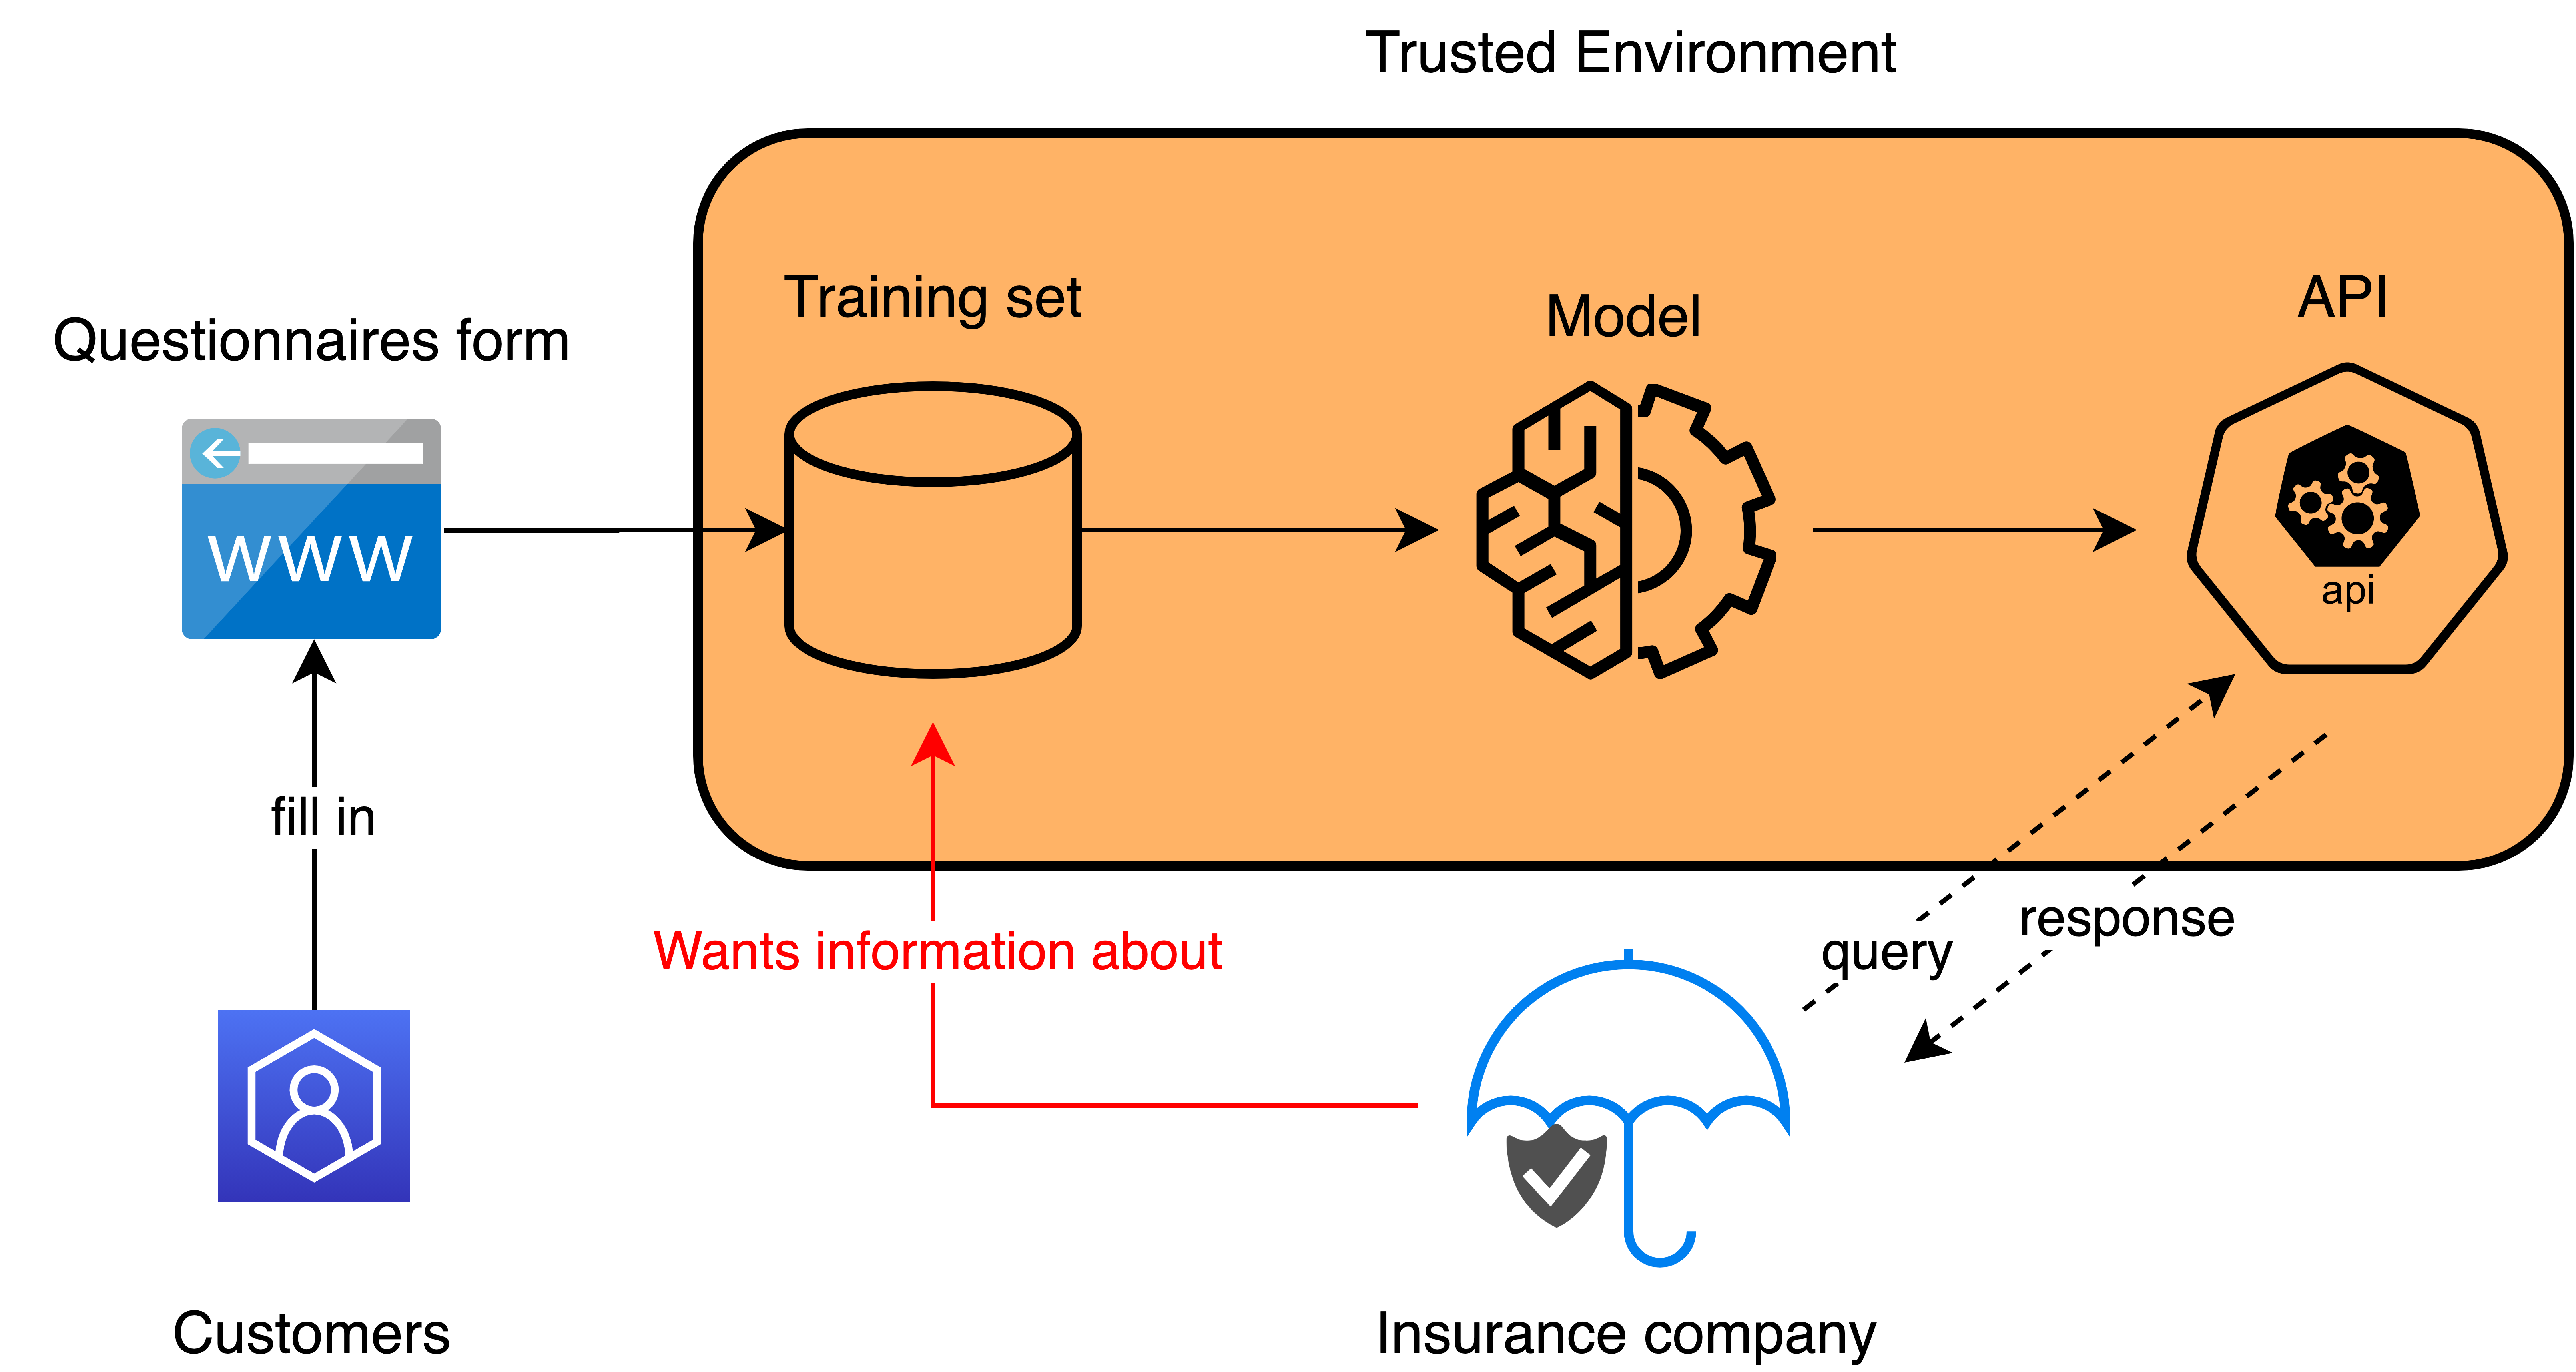
\includegraphics[scale=0.76]{images/introduction/threat_model}
	\caption{\label{fig:threat_model} Threat model}
\end{figure}

In such a model, the insurance company is interested in gaining meaningful information about the training instances that were used by the model. Several attacks can be constructed \cite{ml_survey}:

\begin{itemize}
	\item \textbf{Membership inference attack}: these attacks aim at determining whether or not an input vector $\mathbf{x}$ was used as part of the training set. First introduced by Shokri et al. (2017) \cite{shokri}, it is one of the most popular attacks. This attack assumes a black-box scenario where the attacker only has access to the prediction vectors.
	\item \textbf{Model inversion attack}: given a prediction vector $\mathbf{\hat{y}}$ and partial knowledge of some features of the initial sample $\mathbf{x}$, this attack aims at recovering information about one or all missing features. This is not to be confused with \textit{attribute inference attacks}, which try to infer sensitive feature's values of a targeted instance by leveraging publicly available data.
	\item \textbf{Property inference attack}: these attacks aim at extracting properties over the training set that were not explicitly encoded as features during the learning task. For instance, our synthetic data generation process (described in details in Chapter ~\ref{chap:synthetic_data}) does not encode the number of employees of a company in the dataset. Trying to determine such property from the model would fall under this category of attacks.
	\item \textbf{Model extraction attack}: these attacks do not aim at recovering information about the training dataset, but information about the inner working of the learning model, in order to reconstruct a substitute model that behaves similarly.
\end{itemize}

Many of the above attacks are conducted through \textit{shadow models training}, which is illustrated in Figure ~\ref{fig:shadow}. In shadow training, the attacker trains various models (the so-called shadow models) on shadow datasets, i.e. datasets that follow a similar distribution as the target dataset. Once the shadow models are trained, the attacker constructs an attack dataset, where each instance typically represents the probability vector outputted by the shadow models. The attacker can then train an attack model, which takes as input a prediction vector and outputs membership / property information.

\begin{figure}[h!]
	\center
	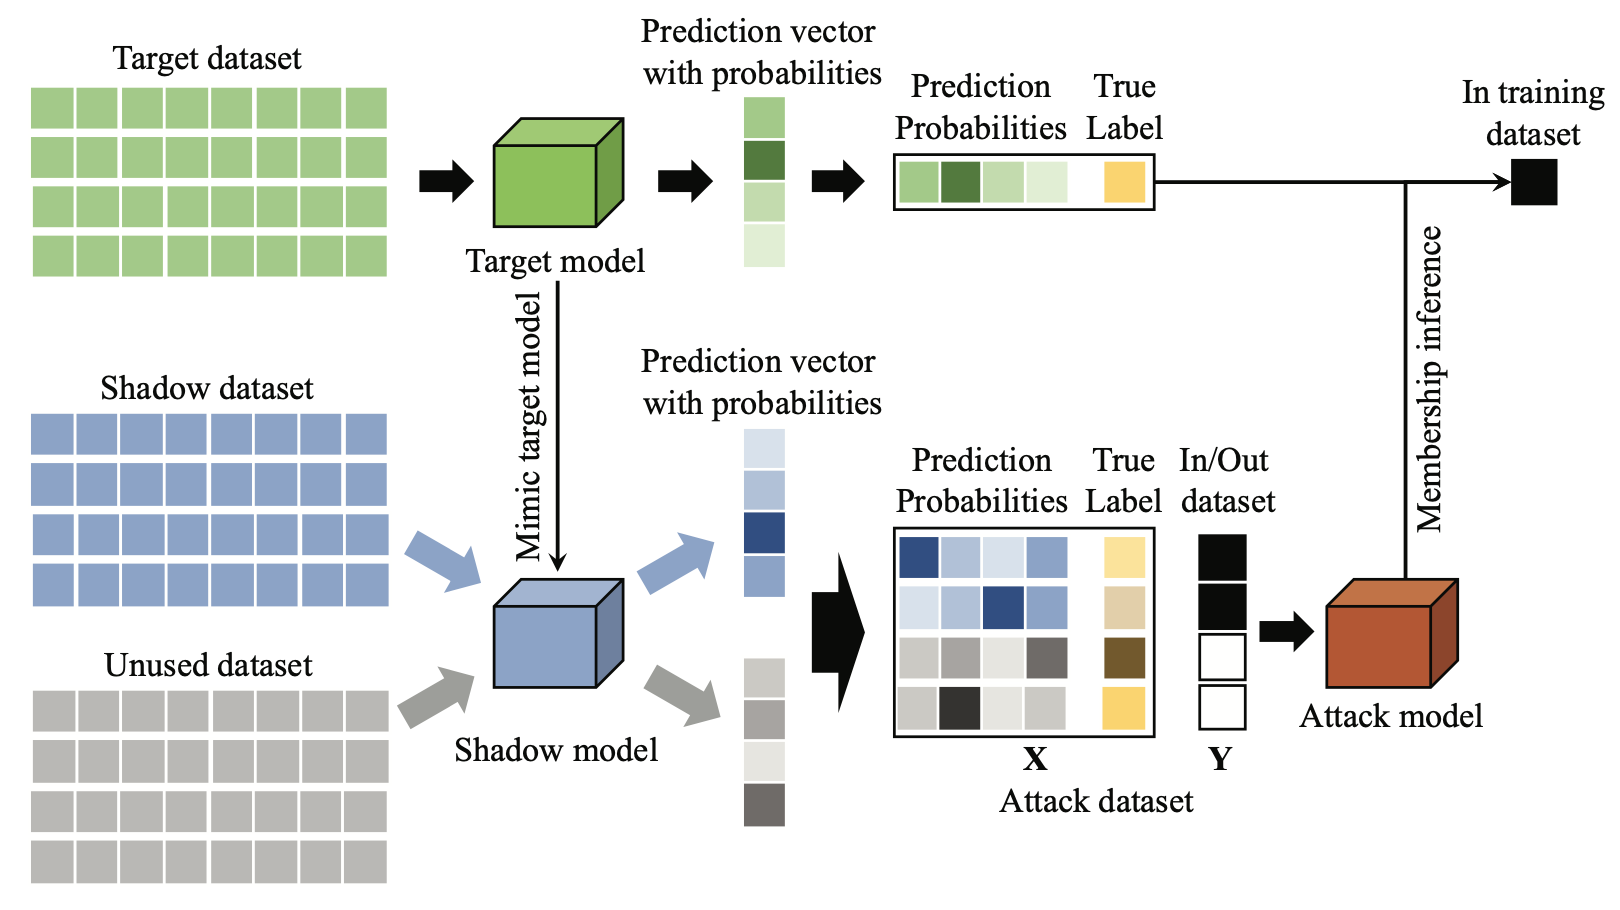
\includegraphics[scale=0.52]{images/introduction/mia}
	\caption{\label{fig:shadow} Shadow training architecture for a membership inference attack. \cite{chen}}
\end{figure}

\section{Attacks on DP-GBDT}

While there are many Python libraries readily available to conduct privacy attacks on machine learning models, such as the \textit{adversarial-robustness-toolbox} Python library\footnote{\href{https://github.com/Trusted-AI/adversarial-robustness-toolbox}{https://github.com/Trusted-AI/adversarial-robustness-toolbox}}, to the best of our knowledge there is no work in the literature that considers privacy attacks on regression models such as our ensemble of gradient boosted decision trees. We therefore tried to convert our synthetic datasets to a classification task, and to tweak our model to support multi-class classification. We evaluate several classical attacks, in particular the gap attack, introduced by Shokri et al. (2017) \cite{shokri}, for different train-test split ratios. Unfortunately, our tests indicate that the current attacks do not adapt well to regression models. In particular, we were unable to detect an explainable correlation between the privacy budget and the accuracy of the membership inference attack. For reference, our results are shown in Figure ~\ref{fig:attack_cost} and summarised in Table ~\ref{table:attack_cost} (for a fixed $\epsilon=0.1$). 

While for low $\epsilon$ values, our model is effectively reducing the success rate of membership inference attacks to $60\%$ or below, the literature (\cite{chen}, \cite{label_only}) shows that we should see such values starting from a higher $\epsilon$ value. Figure ~\ref{fig:attack_cost_50} shows the same attack on a 50-50\% train-test split. From the Figure, what happens is unclear: the model seems not to be leaking any data. However this should be interpreted with a grain of salt, as this could be the result of a lack of better attacks for GBDT models. Indeed, most of current work that evaluates the impact of differential privacy on membership inference attacks targets neural networks and deep learning models only (such as the work in \cite{chen} and \cite{dp_mia}). The reader can refer to Figure 4 in \cite{ref_attack} to get an idea of the influence of differential privacy against membership inference attacks for neural networks.

During this thesis, we have also tried to evaluate the model against other inference attacks, such as attribute inference attacks. Different settings were tested, such as growing very deep decision trees to overfit on the training data. This was done using both the \textit{adversarial-robustness-toolbox} as well as other work found on popular open-source website GitHub. Results were hovering in the 50\% attack accuracy zone, consistently across the different tools, confirming that our model could not be evaluated as-is. This shows that developing privacy attacks on regression ensemble models will be an important step in evaluating them, and we encourage future work in that direction.